\chapter{电力系统结构与状态脆弱性研究分析}
\label{cha:theory}

\section{引言}
\label{sec:index3}

近年来,脆弱性一直是电力系统领域研究的热点。对于电力系统而言,脆弱性的概念目前还没有清晰明确的定义。目前大多数学者认为,电力系统脆弱性是系统本身固有的属性,
在正常运行状态下不会显现。由于电力系统内部结构的复杂性,加之对外部环境的依赖性,在外界扰动或内部结构参数作用下,电力系统的性能参数将会偏离正常范围,影响其电能
质量,因此分析电力系统的脆弱性很有研究意义。

本章将电力系统的脆弱性从两个方面进行展开分析,即结构和状态两个方面,首先从系统整体的脆弱性分析与描述入手,得到清晰合理的电力系统脆弱性本质概念和数学描述;
在此基础上,分别从结构和状态两个方面对系统脆弱性进行分析,在结构方面,主要基于复杂网络和$PageRank$理论进行分析,其脆弱性研究专注于系统受影响的程度;在状态方面,
主要基于蒙特卡洛和概率潮流方法进行分析,其脆弱性研究侧重于抗干扰能力。

\section{电力系统脆弱性分析与描述}
\label{sec:defina}

本节首先对电力系统的稳定性、可靠性以及鲁棒性进行研究分析;在此基础上,结合电力系统脆弱性的特征,得到较为明确的电力系统脆弱性本质概念;进而对电力系统的脆性过程
进行分析,并给出电力系统脆弱性的数学描述。


\subsection{电力系统稳定性、可靠性、鲁棒性的区别与联系}
\label{sec:network}

对于电力系统而言,在进行电力系统脆弱性研究分析之前,有必要明确电力系统脆弱性的概念,不可避免要涉及到系统的稳定性、可靠性以及鲁棒性。这些系统性能概念的提出是为解决
不同的工程实际问题,然而这些概念本身又有相互重叠的部分,因此需要分析电力系统稳定性、可靠性、鲁棒性的概念本质,找出它们之间的区别与联系。并进一步结合电力系统脆弱性的特征,
得到较为明确的电力系统脆弱性概念。

$(1)$稳定性

电力系统的稳定性是当电力系统受到外界扰动时发生的稳定性问题。主要表现在两个方面。当电力系统受到瞬态干扰时,电力系统会偏离原平衡状态,产生偏差,在瞬态扰动消失后,电力
系统可以恢复到原平衡状态;另一方面,当电力系统受到永久性扰动时,如电力系统的节点或线路遭到破坏时,电力系统在经历一个过渡过程后,偏离原平衡状态,达到一种新的平衡状态。
通过上述的定义,电力系统稳定性主要的关注点在于扰动消失后,系统能否恢复到原平衡状态,以及在永久性扰动情况下,系统能否达到新的平衡状态,实现系统稳定运行。

$(2)$可靠性

广义上来说,可靠性是评价元件、产品、系统在一定时间及一定条件下无故障运行的能力或可能性。电力系统的可靠性是指元件、设备或系统在预定时间内,在规定条件下执行规定功能的能力
\cite{refs62}。具体来讲,对于用户而言,电力系统的可靠性是指系统向用户长时间不间断持续提供满足质量要求的电能的能力。这种能力可以通过可靠度、失效率、平均无故障间隔等来
评价。由以上定义可知,电力系统的可靠性主要的关注点在于系统在规定时间内,在规定参数下工作的能力。

$(3)$鲁棒性

鲁棒性一词是原先统计学中的一个专业术语,20世纪70年代才开始在控制理论的研究中流行起来,用来表征控制系统对特征或参数扰动的不敏感性\cite{refs63}。所谓控制系统的鲁棒性是指系统在
自身内部模型不确定性扰动及外部摄动的影响下,系统某个性能指标保持不变的能力。在电力系统中,电力系统的鲁棒性是指系统受到外界扰动或内部自身故障后,系统中绝大部分节点或线路的状
态值保持在稳定裕度范围内变化的能力。也就是说电网中绝大部分节点仍然保持连通。电力系统鲁棒性的主要关注点在于电力系统的抗干扰能力。

通过研究分析系统的稳定性、可靠性以及鲁棒性的定义来看,这三个性能指标的区别如下表所示。

\begin{table}[H]
\centering
\caption{稳定性、可靠性、鲁棒性的区别}
\label{tab:chap3:deference}
\begin{tabular}{C{3cm}C{3cm}C{3cm}C{3cm}}
\toprule
\textbf{系统性能} & \textbf{稳定性} & \textbf{可靠性} & \textbf{鲁棒性}\\
    \midrule
    产生原因       &外部扰动           &外部扰动、内部参数变化         &外部扰动、局部故障\\
    主要关注点     &系统能否回到原平衡状态或能否达到新的平衡状态 
                                          &系统在规定时间和参数下的满足性能运行指标的能力 
                                                                        &系统的抗干扰能力\\
\bottomrule
\end{tabular}
\end{table}

电力系统在稳定性、可靠性和鲁棒性的定义可知,三者的主要关注点上略有不同,如上表所示,然而在产生原因、分析思路和内在概念上,又有着内在的联系。

稳定性是电力系统的基本保障。可靠性是在稳定性的基础上,针对具体的性能指标,可靠性强调的是在规定时间保持规定指标要求运行的能力。鲁棒性是在稳定性的基础上,研究在外界扰动或发生
局部故障后,系统性能参数保持在稳定裕度范围内的能力。

与鲁棒性概念有一点类似,不同之处在于,一是脆弱性是电力系统固有的属性,任何一个电力系统都存在脆弱性,系统正常运行的情况下,不会显现;二是其耐受程度不但包括系统抗干扰的能力,还
包括系统受影响的程度;三是电力系统的脆弱性包括结构脆弱性和状态脆弱性两个方面。电力系统可靠性概念可为研究系统状态脆弱性指标提供借鉴的思路。


\subsection{电力系统脆弱性的本质及脆弱过程分析}
\label{sec:network}

经过上一节对电力系统性能的研究分析后,结合第二章对复杂网络脆弱性概念的描述,本节对电力系统脆弱性的本质概念进行如下定义与描述。

电力系统作为复杂系统中的一种典型系统,其脆弱性是系统本身固有的一种属性,在正常运行和工作状态下不会显现。在电力系统中,每个子系统或元件是相互关联的,当子系统或单个元件由于外界
扰动或自身参数变化而使正常运行状态改变时,会导致系统承受不确定性因素的能力变差,这种特性即为系统的脆弱性。它表现的是系统对外界扰动或自身参数变化的耐受程度。其耐受程度由两个
方面的体现,一是系统受影响的程度;二是系统抗干扰的能力。

电力系统耐受程度可通过系统性能指标进行分析,当外部扰动或内部参数改变时,系统的性能指标在稳定裕度范围内变化,说明系统的耐受程度高,系统脆弱性差,反之,系统性能参数超出稳定裕度范围,
系统性能变差,系统脆弱性强。

按研究角度的不同,将电力系统的脆弱性分为结构脆弱性和状态脆弱性。结构脆弱性研究的是电力系统中某个元件在网络拓扑的重要程度;状态脆弱性则研究的是电力系统各状态变量偏离正常运行状态
及距离临界状态的程度。

随着电力系统拓扑结构复杂性的提高,负荷需求的增大,加之影响电力系统脆弱性的因素复杂多样。电力系统在局部故障发生后,由于级联特性,极易出现连锁故障,进而导致大面积网络瘫痪。
因此有必要对脆弱性过程进行深入分析。电力系统脆弱性激发过程如下:
\begin{figure}[H] % use float package if you want it here
  \centering
  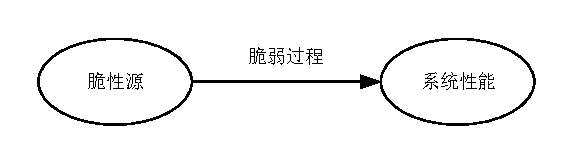
\includegraphics[]{cuiruo_Processoin.pdf}
  \caption{脆性源、脆性过程及系统性能的关系图}
  \label{fig:procession}
\end{figure}

脆性源:包含系统脆弱性的元件(节点或线路)。当脆弱性条件触发时,脆性源会将脆性发出,进而引发其他部分的崩溃,这部分元件称为脆性源。其脆弱性触发条件有很多,如元件状态参数、
结构参数的变化。

脆性过程:在电力系统中,脆性过程为脆性源激发后,其脆弱性的传递过程,由于电网的级联效应,会导致系统性能参数的变化和连锁故障的发生。

系统性能:表征的是系统保持正常运行的能力,通常会定义系统性能指标来评估脆性源对系统整体性能的影响程度。

通过对以上三个环节的定义与描述,本文对电力系统的脆弱性过程进行如下阐释:

当脆性源的脆弱条件触发时,脆性源会被激发,将电力系统的脆弱性发出,由于电网的级联效应,在脆性过程环节其脆弱性会被传递,使得系统的性能参数发生变化(拓扑完整性
变差和状态参数偏离正常范围)。脆性源、脆性过程和系统性能三个环节在一个过程中同时激发,这构成了电力系统的脆弱性传递过程,三者缺一不可。

在本文中,通过对电力系统脆弱过程的分析,主要研究两个方面的内容:

$(1)$通过分析脆性源,研究脆性的触发条件,对系统的脆弱节点进行判断和识别,通过安全策略加强对脆弱环节的保护,从源头降低系统脆弱性传递的可能性。这也是本文研究的重点。

$(2)$通过分析脆性源对系统性能的影响,研究系统节点的脆弱性评价指标,评估脆弱节点对系统性能的影响程度。以此作为识别脆弱环节的重要参考。



\subsection{电力系统脆弱性的数学描述}
\label{sec:describtion}

通过对电力系统脆弱性本质概念的分析研究可以得出,对于电力系统而言,系统性能变化的主要原因是外部扰动对系统元件的影响以及元件内部结构参数的变化,即脆弱源。脆弱源作用于脆弱环节,使得
系统脆弱性凸显,系统性能变差。

设系统$S$由$n$个元件$C_i$组成,且$C_i$的状态用$x_i$表示,$x_i \in X \subset R^m$。如果存在一个元件$C_b$,当其结构或状态发生变化,使得$x_b \to x_B$,有
\begin{equation}
  \lim _{g\left(x_{0}\right) \rightarrow G\left(x_{s}\right)} \delta(s) \neq \delta\left(s^{-}\right)
  \end{equation}
 
式中,$\delta\left(s^{-}\right)$为系统初始稳态的性能指标,$B$为元件$C_B$的不稳定域,$G\left(x_{B}\right)$为$C_B$不稳定域的阈值函数,$g(x_b)$是衡量$C_b$元件的性能指标,
$\delta\left(s\right)$为当前系统$S$的性能指标。

复杂系统是由元件、关系、环境组成的,元件在电力系统中对应着母线节点和线路,关系对应着节点之间的连接情况和潮流分布流向,环境对应的是一切影响电力系统结构或状态参数原因的集合。研究电
力系统的脆弱性,主要就是研究在不确定的环境中各元件之间、元件与整体之间、元件与环境之间以及整体与环境之间的内在关系,本文的主要研究方向是电力系统的节点或线路受到不确定因素影响后结
构或状态发生变化,对其他元件和整个系统产生的影响。

可以看出,系统脆弱性的数学描述和定义主要在于元件的存在性对于整个电力系统的影响,即存在能够引起整个系统性能改变的元件,量化系统中的元件对整个系统的重要程度,以及如何识别出这样的元件
是电力系统脆弱性研究的一个重要方向,通过加强对脆弱环节的重点保护和电网拓扑的优化改进,从而为预防大规模停电事故和连锁故障的发生提供了参考方向。


\section{电力系统结构脆弱性研究}
\label{sec:construction}

电力系统的结构主要是指由发电节点、负荷节点和传输线路组成的网络拓扑。拓扑结构是电能传输和系统性能的基础,它决定了电能是否能够被安全、可靠、有效地从发电节点传输到负荷节点。当电力系统
拓扑结构保持完整时,是保证电力系统稳定可靠运行的基础。但是,受外界环境的干扰,人为因素和保护设备内部故障等原因的影响,拓扑结构的完整性会受到破坏,导致电力系统无法安全可靠运行,甚至
崩溃。因此,有必要分析各个节点在网络拓扑的重要程度,进而加强对重要节点的防范和预先保护,对电力系统的稳定、高效、可靠运行有重大意义。

\subsection{电力系统结构脆弱性的定义与数学描述}
\label{sec:network}

电力系统的结构脆弱性是指电力拓扑结构中节点或线路由于外界或内部因素的影响下,导致节点或线路发生故障断开后,电网保持其连通性和维持基本稳定运行状态的能力,即保持拓扑结构完整的能力。

在电网拓扑结构方面可选取一定的评估指标,来考察某一单元或某些单元退出后系统的耐受程度——系统受影响的程度。对系统结构影响程度大的节点或线路,说明其对网络拓扑结构的完整性贡献程度高,
对于这样的节点或线路称为系统结构的脆弱点。因此,可以认为对电力系统拓扑结构影响越大的节点或线路,其脆弱性程度越高。

结构脆弱性研究的是电力系统中某个单元在网络拓扑的重要程度。在电力系统拓扑结构方面,从不同方面研究得到的结构脆弱性的指标描述不同,每个方面都有其结构重要性指标来衡量一个元件$i$在系统
中的重要程度,其数学描述如下:
\begin{equation}
  A(i)=\sum_{j\in F(i)}{k(i,j)}
  \end{equation}

$F(i)$为元件$i$有关联的元件的集合,$k(i,j)$为从不同角度考虑得到的结构脆弱性表达式,表示$i$和$j$在拓扑结构上的联结程度。

% 将$A_l(i)=\sum_{j \in F(i)}{k_l(i,j)}$定义为从某一方面考虑的结构脆弱性描述,那么从各个方面考虑的结构脆弱性数学描述定义为结构矩阵$Z$,$Z=[A_1,A_2,A_3\cdots A_n]]$于是结构脆弱性
% 矩阵的数学描述为


\subsection{基于复杂网络的结构脆弱性研究}
\label{sec:network}

复杂网络的基本思想是将一个复杂系统抽象为网络,其中系统中的单个元件被视为网络的节点,而元件之间的联系被视为网络的边,由此建立复杂网络模型。基于传统的复杂网络理论,电力系统中的母线
可以被视为节点,母线之间的传输线路被视为边,线路上的阻抗被视为权重,因此整个电力系统等效为加权无向图\cite{refs64,refs65}。

在本文2.2中,复杂网络理论描述网络的特征参数有特征路径长度、节点度和节点度分布、聚类系数、介数和介数分布等。参照复杂网络特征参数定义,并结合电力系统的特点,定义“电气度”概念如下:
\begin{equation}
\label{equ:chap3:index1}
  e_{i}=\sum_{j=1, j \neq i}^{N} e a_{i j} \cdot e w_{i j}
  \end{equation}

式中,$e a_{i j}$为网络中邻接节点的连接情况,为 0 代表$i$,$j$不相连,为1代表$i$,$j$相连。而$ew_{ij}$代表支路潮流上的视在功率的大小。电气度指标综合考虑节点连接数量和连接强度,
衡量的是节点在拓扑形结构中承担应力的大小,是网络中衡量节点重要性的重要参数。

介数作为复杂网络的关键参数之一,被用来描述节点或者边在信息、能量传递中的重要程度。介数的概念在电力系统被称为电气介数,它反映了网络节点、支路在整个电能输送过程中的贡献程度\cite{refs66,refs67}。

假设一个电网具有$a$个母线节点,$b$条电气连接的边,那么支路$l_{mn}$的电气介数计算公式如下:
\begin{equation}
\label{equ:chap3:cb}
  C_{B}(m, n)=\left|\sum_{i \in \mathrm{G}, j \in \mathrm{D}} w_{i j} P_{m n}(i, j)\right|
  \end{equation}

式\ref{equ:chap3:cb}中,$G$,$D$分别为发电节点、负荷节点的集合。$P_{mn} (i, j)$是单位有功功率注
向发电节点$i$和负荷节点$j$时,支路$l_{mn}$ 上产生的有功功率。$w_{ij}$是发电节点$i$和
负荷节点$j$的节点对间传输电能的权重值,大小为$min(|P_i|,|P_j|)$,分别代表了发
电节点$i$在发电节点功率总和的比率和负荷节点$j$在负荷节点功率总和的比率。

电网中节点的分类分为发电节点,负荷节点,中间节点。所有的功率都是从发电节点向负荷节点传输,因此需要对上述公式进行修正得到如下的节点电气介数计算公式。
\begin{equation}
\label{equ:chap3:cb1}
C_{B}(k)=\left\{\begin{array}{ll}{\frac{1}{2}\left(\sum_{l \in \mathbf{F}(\mathbf{k})} C_{B}(k, l)+\sum_{i \in \mathbf{D}} w_{k i}\right),} & {k \in \mathbf{G}} \\ 
{\frac{1}{2}\left(\sum_{l \in \mathbf{F}(\mathbf{k})} C_{B}(k, l)+\sum_{i \in \mathbf{G}} w_{i k}\right),} & {k \in \mathbf{D}} \\
 {\frac{1}{2}\left(\sum_{l \in \mathbf{F}(\mathbf{k})} C_{B}(k, l)\right)} & {k \notin \mathbf{G}, k \notin \mathbf{D}}\end{array}\right.
\end{equation}

式\ref{equ:chap3:cb1}中,
$F(k)$指的是与节点$k$相连的所有边的集合,$C_B (k,l)$为对应支路的电气介数。节点的电气介数与拓扑中所连支路的电气介数有直接关系。

由此所有节点的电气介数计算流程图如图\ref{fig:nodeBetweenPro}所示。 
\begin{figure}[H] 
  \centering
  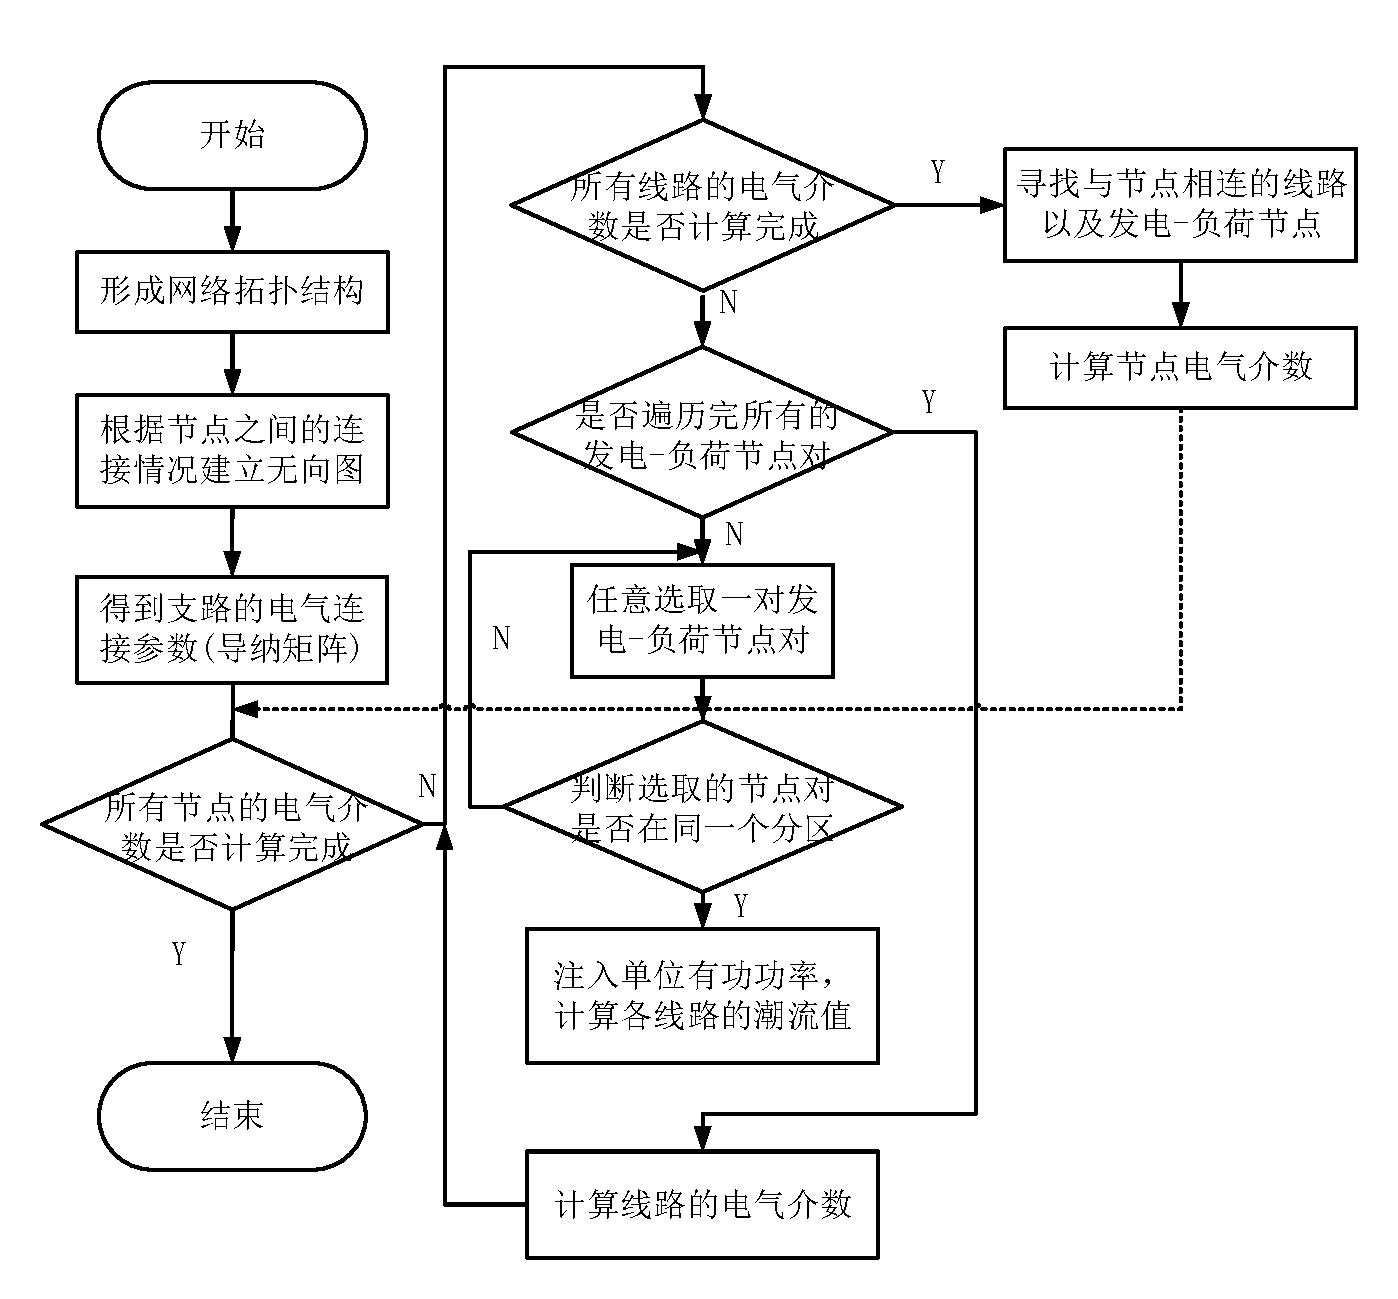
\includegraphics[height=12.7cm]{nodeBetweenProcess.pdf}
  \caption{电气介数计算流程}
  \label{fig:nodeBetweenPro}
\end{figure}

从流程图可以看出,节点的电气介数综合考虑了所连支路对其的影响。而支路的电气介数则衡量了所有发电-负荷节点对支路潮流的影响,从而在分析时,
不仅考虑了拓扑的影响而且增加了能量变化的考虑,使得结构的衡量更完善。电气介数不局限于能量、信息沿着网络的最短路径传播,更体现了电能在整个网络
支路的分布情况。同时,电气介数还分别考虑了发电节点和负荷节点的变化影响,改变他们的容量,网络各节点的重要性也会发生变化,因此,电气介数更符
合实际电网的变化情况。




$PageRank$最早是被用来作为互联网网页结构的模型,并且对所有网页进行重要度排序的一种算法\cite{refs68,refs69}。在众多计算互联网网页的相关性的算法中,$PageRank$是名气最大,
且最早被谷歌浏览器采用的。$PageRank$的基本思想是一个网页的重要性依赖于所有链接向它的其他网页。比如,网页$i$有链接指向网页$j$,如果有很多其他网页有链接指向网页$j$,那么我们认为
,网页$j$是非常重要的。另一方面,若只有一个网页有链接指向网页$j$,由于这个网页是一个权威性很高的网址,如谷歌,百度等网页,我们认为网页$j$也非常重要,因为由受欢迎、权威的网页指向它,
这份重要性将会传递下来。

在复杂系统理论中,$PageRank$算法的思想是将复杂系统等效为一个有向图。本文将电网与互联网网页搜索结合,将电力系统抽象成有向网络图,电网中,每条支路上的潮流是有确定的方向的,
所以可以被视为一个有向图。每个母线节点被视为一个网页,母线节点之间的电气连接被视为网页中的超链接,根据潮流的方向决定超链接的方向。互联网与电网的$PageRank$的拓扑模型比较
如表~\ref{tab:PRComparision}。在已有的研究中,在$PageRank$模型的网页出链的处理上采用均分的思想\cite{refs70},本文在综合考虑潮流能量对结构的影响下,认为出链是按照实际
的潮流的比重进行分配的。

按照网页的超链接可以传递重要性的思想,假设$A$节点拥有~3~个出链,它会分别按照视在功率的比例分别传递给所指向的$B$、$C$、$D$三个节点,按照潮流能量的分布作为权重。根据重要性传递规则,
可以得到能量转移矩阵$A$。对于没有出链的节点,则按照$PageRank$的算法,认为该节点对所有节点都出链,从而解决终止点的问题。因为电网的潮流能量分布中不存在自己指向自己的连接,故不存在
陷阱问题,因此不予考虑。
\begin{table}[htb]
  \centering
  \caption{互联网与电网的$PageRank$拓扑模型比较}
  \label{tab:PRComparision}
    \begin{tabular}{C{4.5cm}C{4.5cm}C{4cm}}
      \toprule
      互联网 & 电网 & $PageRank$拓扑 \\
      \midrule
      网页 & 母线 & 节点\\
      超链接 & 输电支路 & 有向边\\
      指向该网页的网页数目 & 母线进线数目 & 入度\\
      该网页指向的网页数目 & 母线出线数目 & 出度\\
      \bottomrule
    \end{tabular}
\end{table}

$PageRank$算法应用于电网拓扑的具体步骤为:

$(1)$假定初始服从均匀分布,即每个母线节点的重要性都是相同的,即对于一个一共有$n$个节点的系统而言,赋予每个网页初始相同的$PR$值,一般都为1。

$(2)$根据电网的实际潮流计算每条连接上的视在功率得到能量分布权重的矩阵P,再根据公式\ref{equ:chap3:Index3}得到能量转移矩阵A。

$(3)$迭代计算,由于每个超链接的存在都会增加对应网页的$PR$值,所以通过考虑潮流连接、能量转移情况对各个母线节点的$PR$值进行迭代更新。

$(4)$最后,经过若干次的迭代后,各个母线节点的$PR$值会趋于一个稳定的值。
\begin{equation}
\label{equ:chap3:Index3}
PR(p_i)=\frac{1-q}{N}+q\sum\limits_{p_j\in\mathbf{M_{p_i}}}{\frac{PR(p_j)}{L(p_j)}}
\end{equation}

式~(\ref{equ:chap3:Index3})中,$p_i$是被计算的节点,$M_{p_i}$是节点$p_i$的入链节点集合,$L(p_j)$是节点$p_j$的出链数目,$N$是节点总数目。$q$为阻尼系数,一般取~0.85~,引入该参数是为了解决出链为零的节点在模型计算中带来的问题,代表了当前的母线节点没有遭到破坏正常运行的概率。$1-q$则代表了节点遭到意外破坏退出运行的概率。从公式中可以看出,$p_i$节点的$PR$值与和它相连的$p_j$节点的$PR$值有关,其值越大,且$p_j$节点的出链越少,$p_i$节点的$PR$值越大。其计算流程图如下:
\begin{figure}[H] % use float package if you want it here
  \centering
  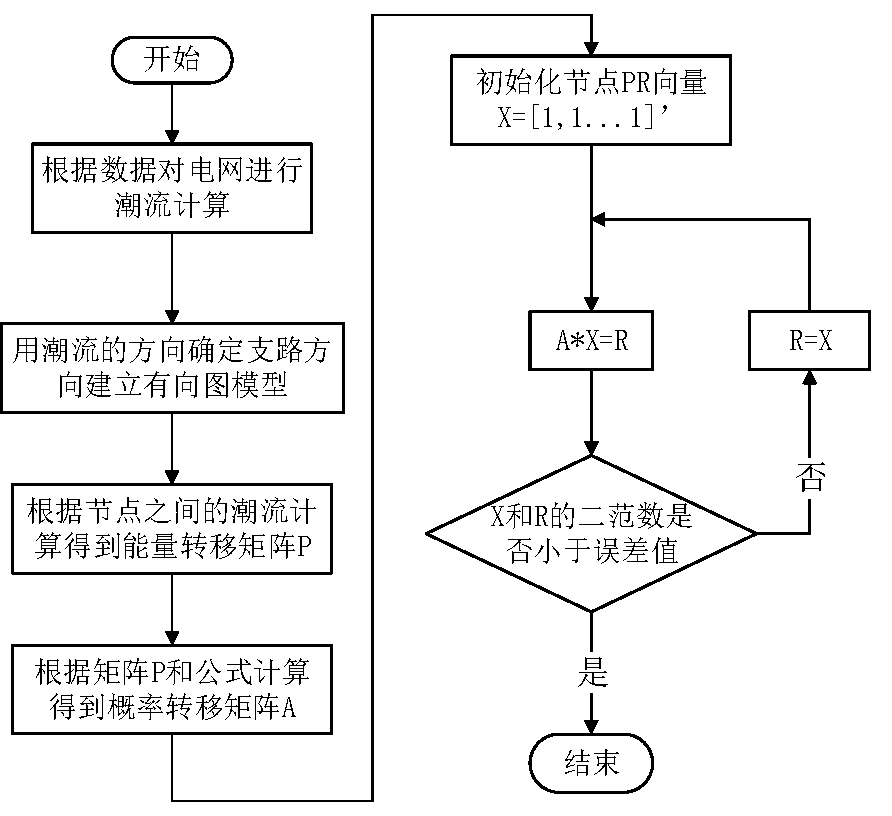
\includegraphics[height=8.4cm]{PRprocess.pdf}
  \caption{$PangRank$计算流程}
  \label{fig:PRPro}
\end{figure}

由图可知在$PageRank$在计算中,考虑更多的是节点的重要性在拓扑中的传递性。即通过反复迭代,确保所有节点的$PageRank$值在整个拓扑的重要性分配中趋于稳定,误差达到最小。$PR$值代表了节点在网络中的重要程度,$PR$值越高,节点越重要。

\subsection{模型比较与案例分析}
基于前面的研究可知,对电力系统的拓扑建模有两种不同的角度。不考虑潮流的方向,关注支路的重要性可将系统视为一个加权无向图。反之,考虑潮流的方向,衡量出入链对结构的影响可将系统视为一个有向图。复杂网络的电气介数更多关注的是支路上的潮流分布对拓扑重要性影响,而$PageRank$算法则更多关注的是有向的连接关系对拓扑重要性的影响。本节以$IEEE14$数据集为例,分别用以上的两种方式建模。该电网拓扑原理图如下:
\begin{figure}[H] % use float package if you want it here
  \centering
  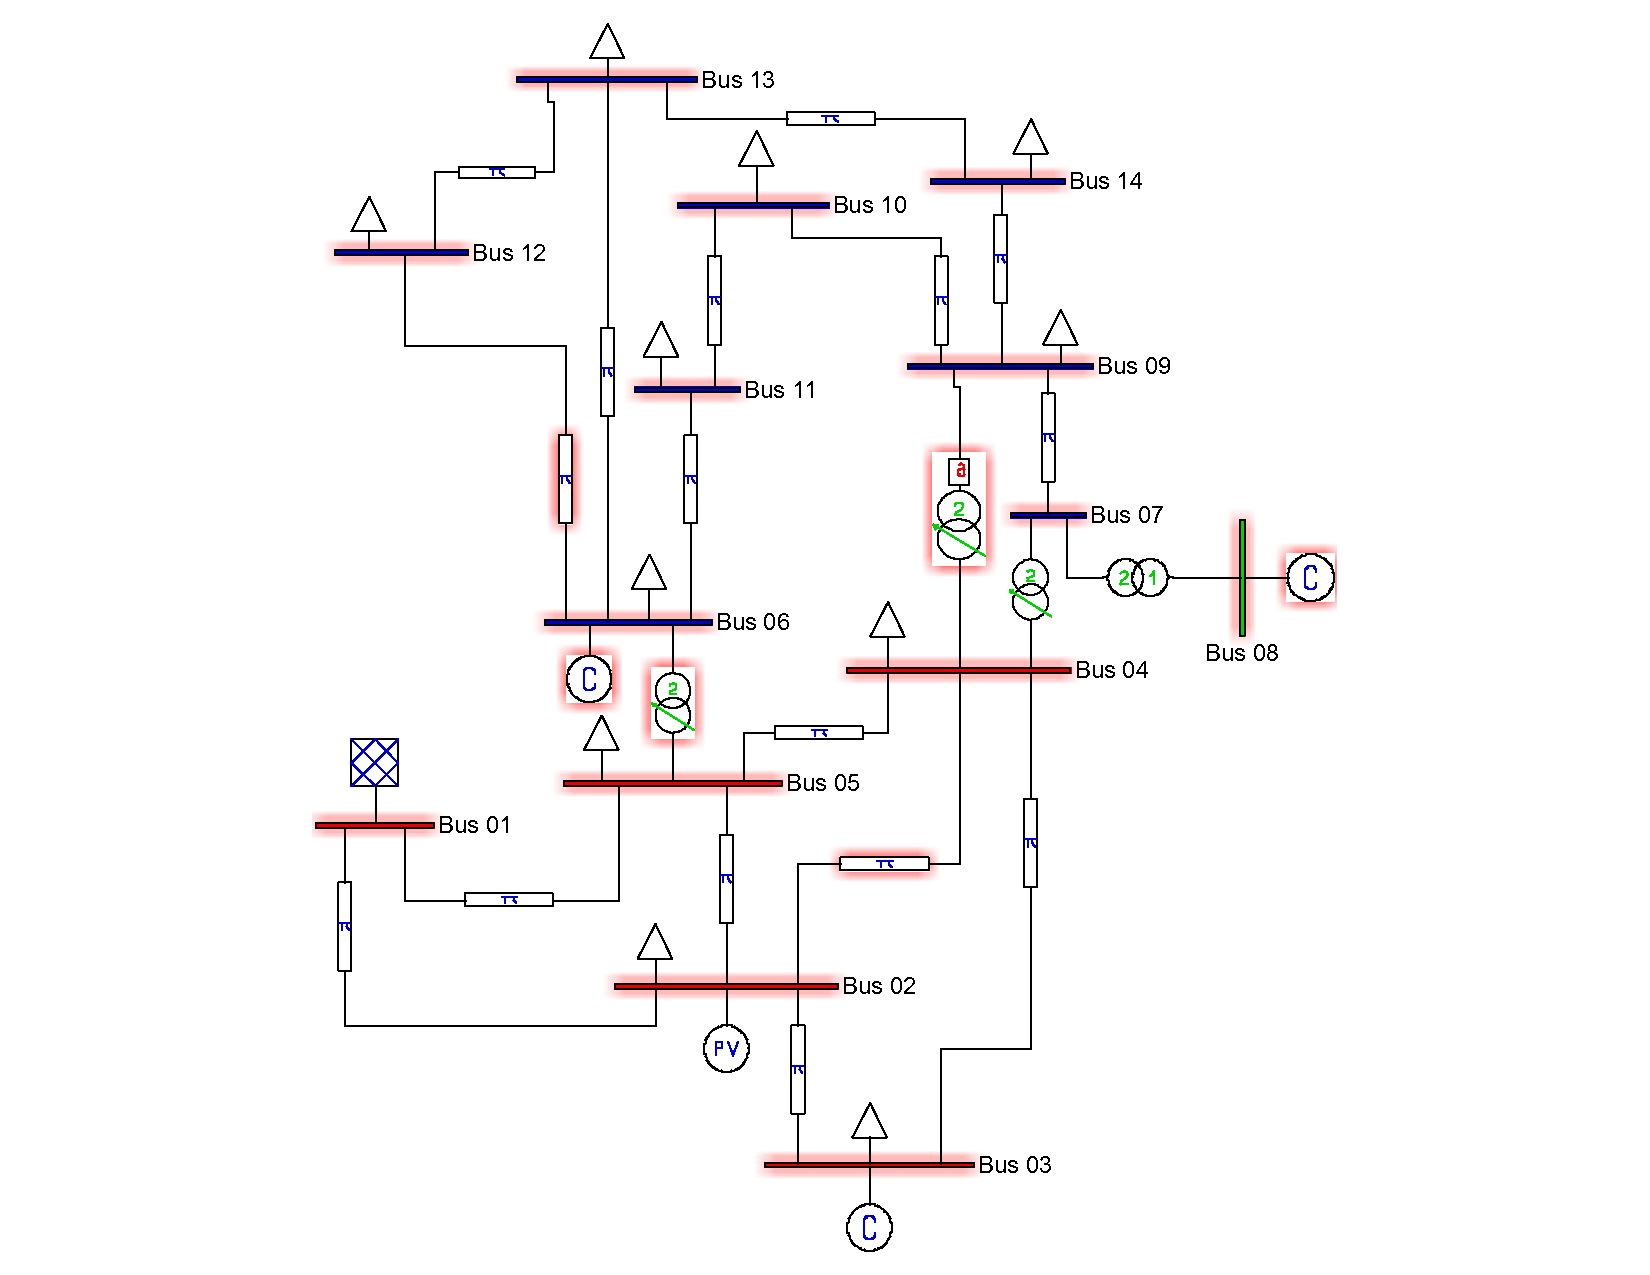
\includegraphics[height=13cm]{IEEE14.pdf}
  \caption{$IEEE14$电网拓扑原理图}
  \label{fig:fundement14}
\end{figure}

针对该拓扑,复杂网络的建模将其等效为一个无向图如图\ref{fig:model1},图中按照支路电气介数的大小等比例加粗了图的边,再根据图中的流程\ref{fig:nodeBetweenPro}最终计算得到各个节点的电气介数。电气介数计算的过程中,节点的电气介数直接受支路的电气介数影响。而支路的电气介数计算突出的是支路结构对能量分布的影响,能量分布越大的支路其电气介数也相应的越高。而$PangRank$的建模则将其等效为一个有向图如图\ref{fig:model2},再根据图\ref{fig:PRPro}最终计算得到各个节点的$PR$值。$PangRank$计算的过程中,突出的是拓扑的出入链的重要性。对于该模型,其迭代过程在能量转移矩阵的作用下完成,而入链累计度越高的点的$PangRank$越高。$PangRank$衡量了拓扑节点在能量转移中所起的作用。
\begin{figure}[H]
\begin{minipage}{0.48\textwidth}
  \centering
  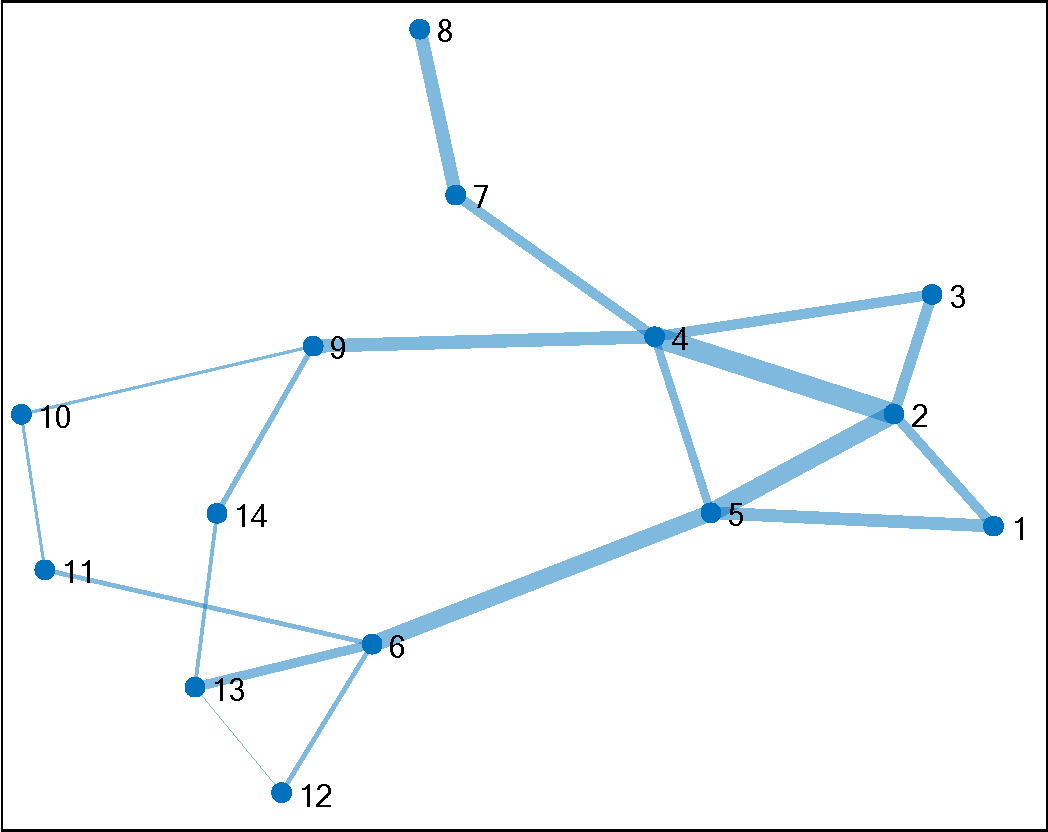
\includegraphics[height=5.8cm]{graph14.pdf}
  \caption{基于复杂网络的拓扑建模}
  \label{fig:model1}
\end{minipage}\hfill
\begin{minipage}{0.48\textwidth}
  \centering
  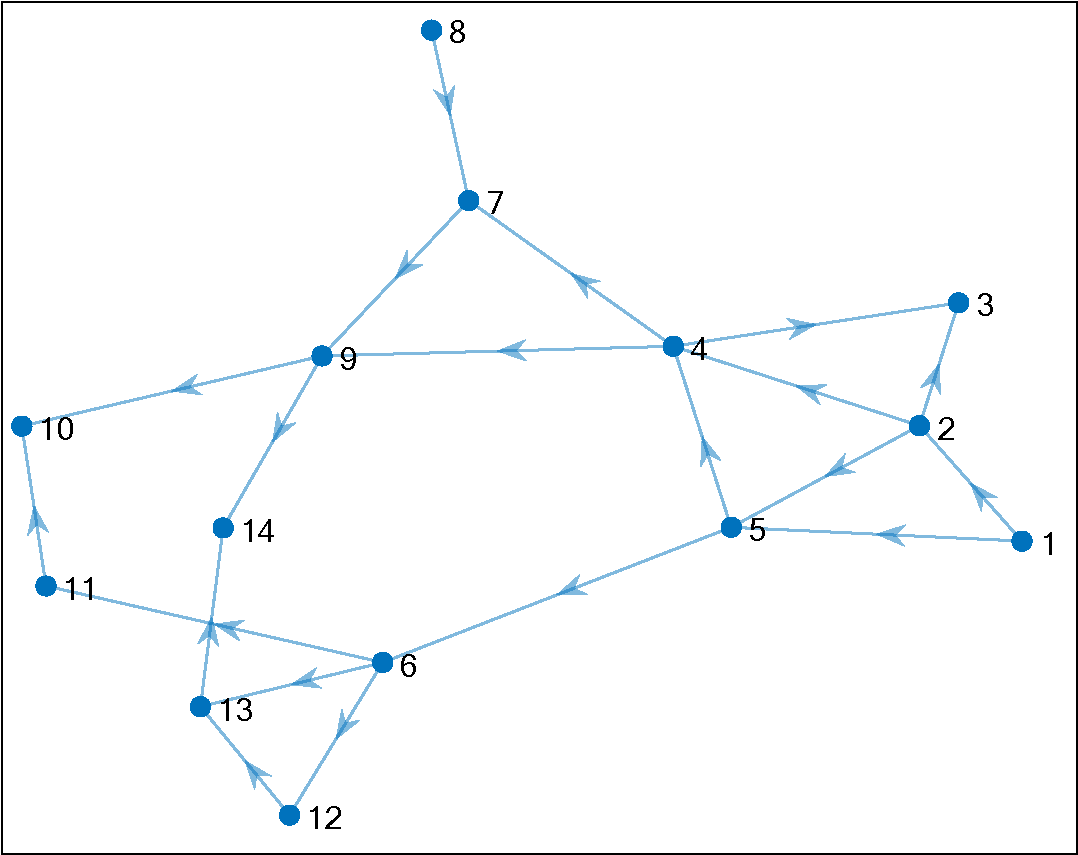
\includegraphics[height=5.8cm]{disgraph14.pdf}
  \caption{基于$PageRank$的拓扑建模}
  \label{fig:model2}
\end{minipage}
\end{figure}
电气介数与$PangRank$计算结果比较如图\ref{fig:compare_nodePR}。由于两个指标基于的拓扑模型不同,所以计算的结果相差较大。首先分析复杂网络的模型,从图中可以看出,支路的电气介数直接影响到了节点的电气介数,比如$2$、$4$、$5$节点由于与节点相连的支路比较重要而对拓扑具有较大的影响力。而支路的重要是因为$1$、$2$、$3$、$6$是系统中的发电节点,其功率传输分布因子较大,故而电电气阶数较大。而$4$、$5$处于发电和负荷的中间传输点,承担了较大的传输潮流的作用,因此相连的支路的电气介数都较大。$8$由于发电功率几乎为零且所连支路只有一条所以电气节数很小。而$12$、$11$、$10$负荷节点相连的支路都不是主要输送支路,功率传输因子小,所以电气节数较小。

反观$PangRank$的模型,该模型将每个节点的重要性赋予在该节点指向其他节点的出链上,因此,那些入链累计度高的节点重要性也高。比如$14$、$10$、$9$,这些节点均是负荷节点,能量最后传输给负荷,由于被潮流指向的累计的节点较多,即该节点的入链节点的入链节点数较多,因此重要性的权重被累计、叠加的程度较大。这种模型也符合现实,实际情况中,能量被输送、汇集到负荷节点,而负荷节点直接与用户相连,直接影响配电质量。因此,负荷节点在结构中的重要性非常高。在$PangRank$的模型中,由于发电节点是潮流起始点,$1$、$8$节点不仅是发电节点,而且是单向输出,没有其他入链,所以其$PR$值较小。

综上分析,电气介数与$PangRank$均对电力系统的结构特点进行了描述,均反映了各个节点在拓扑中的重要程度:前者从能量传输分布的角度对系统的拓扑进行了研究,后者从潮流累计分布的角度对拓扑进行了分析。因此,本文在第四章中将这两个指标进行了融合分析,作为结构脆弱性的综合评价指标。

\begin{figure}[H] % use float package if you want it here
  \centering
  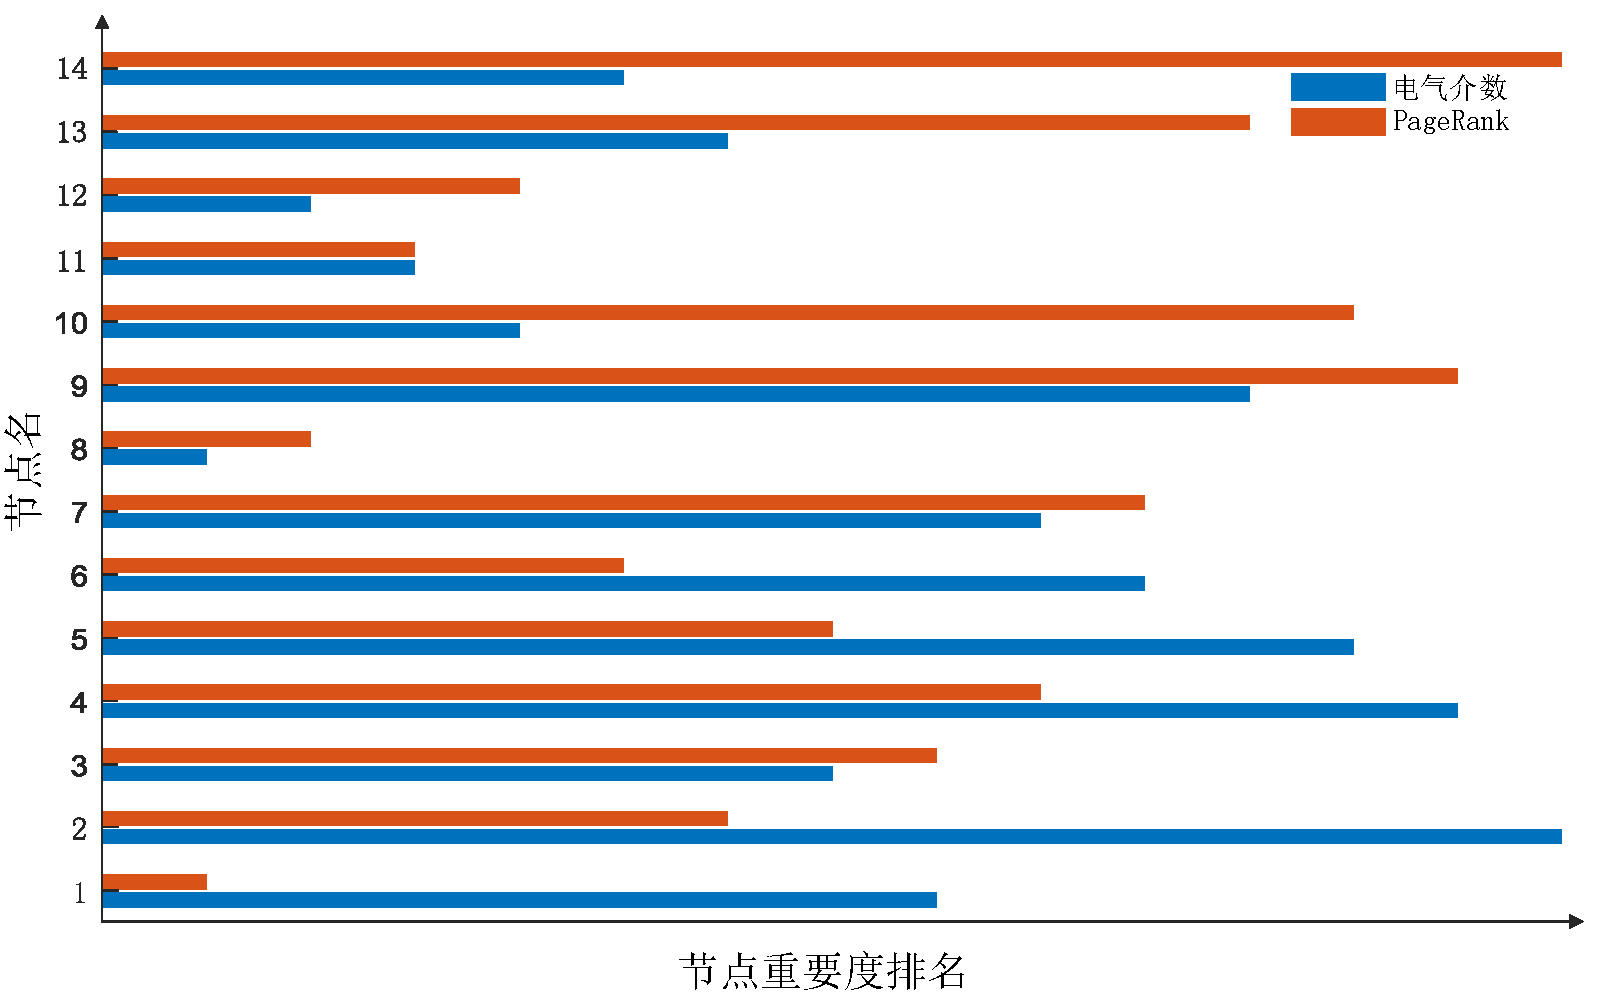
\includegraphics[height=8.7cm]{compare_nodePR.pdf}
  \caption{电气介数与$PangRank$计算结果比较图}
  \label{fig:compare_nodePR}
\end{figure}

\section{电力系统状态脆弱性研究}
\label{sec:status}

电力系统运行中,每个节点或线路都有其对应的状态变量,对电力系统而言,环境的变化会导致系统运行状态变化。环境的变化主要体现在发电节点发电容量的变化和负荷节点的负荷容量变化。
因此在电力系统状态研究中,潮流计算扮演了重要的角色。在系统的运行状态发生改变改变时,电力系统潮流分布进行重新分配。电力系统的潮流计算是计算每一种运行状态下系统的运行参数,
如电压、功率和相角等,进而判断各个运行参数是否在安全裕度范围内运行,潮流的分布是否合理是潮流计算的基本目标。


\subsection{电力系统状态脆弱性的定义与数学描述}
\label{sec:vulneStaus}

电力系统的状态脆弱性是指系统在受到外界扰动或内部自身故障后,节点或线路的状态变量发生变化,并由初始状态(额定状态)向临界点逼近的特性。表现了某个节点或线路从稳定状态向临界失稳
状态的过渡过程。反映了系统的抗干扰能力,在扰动作用下,节点或线路当前运行状态距离临界状态越大,说明其越难达到失稳状态,系统的抗干扰能力越强。本文认为,在扰动作用下,电力系统中
的节点或线路的运行状态值越接近临界失稳值,其脆弱程度越大,越易影响系统的正常运行。

状态脆弱性研究的是电力系统各元件状态变量偏离正常运行状态及距离临界状态的程度。电力系统的状态量包括功率、电压、相角等。其分析方法与传统的稳定性分析方法比较接近,数学描述如下:
\begin{equation}
\Delta \alpha=\left|\alpha(t)-\alpha\left(t_{0}\right)\right|  
\end{equation}

式中:$\alpha(t)$表示节点或线路状态变量当前值,$\alpha\left(t_{0}\right)$表示节点或线路状态变量初始值(额定值),$\Delta \alpha$表示当前状态值相较于初始状态值的偏离程度。
用$\Delta \alpha_i$表示元件$i$的状态偏离程度,则电力系统各元件的状态偏离矩阵为:$D=\left[\begin{array}{lll}{\Delta \alpha_{1},} & {\Delta \alpha_{2},} & {\Delta \alpha_{3} \cdots \Delta \alpha_{n}}\end{array}\right]$

% \begin{equation}
% D=\left[\begin{array}{lll}{\Delta \alpha_{1},} & {\Delta \alpha_{2},} & {\Delta \alpha_{3} \cdots \Delta \alpha_{n}}\end{array}\right]
% \end{equation}

电力系统元件的状态偏离程度还可用百分比的形式进行表示:
\begin{equation}
  \theta=\left|\frac{\alpha(t)-\alpha\left(t_{0}\right)}{\alpha_{m}(t)-\alpha\left(t_{0}\right)}\right|
  \end{equation}

式中:$\alpha_{m}(t)$为元件状态变量的临界值,$\theta$为状态变量当前与初始稳态值的差值与临界偏差量的百分比,它表示状态的变化量相对于临界偏差的偏离程度。当$\theta<1$时,表示
元件处于正常运行状态;当$\theta>1$时,表示元件偏离临界值,元件处于失稳状态。那么电力系统各元件状态的变化量相对于临界偏差量偏离矩阵为:$E=\left[\begin{array}{lll}{\theta_{1},} & {\theta_{2},} & {\theta_{3} \cdots \theta_{n}}\end{array}\right]$

定义$f\left(\alpha_{1}, \alpha_{2}, \alpha_{3} \cdots \alpha_{n}\right)$为节点$i$或线路$i$状态变量当前值的关联函数,某一状态变量变化导致关联函数变化,当节点或线路$i$当前
状态值发生变化,其关联函数相对当前状态值变化的比值可用如下偏导式进行表达:
\begin{equation}
  \varphi=\frac{\partial f}{\partial \alpha_{i}}
  \end{equation}
将$\varphi$定义为状态灵敏度,表示当前状态值的改变对关联函数的影响程度。那么,电力系统各元件的状态灵敏度矩阵为:$F=\left[\begin{array}{lll}{\varphi_{1},} & {\varphi_{2},} & {\varphi_{3} \cdots \varphi_{n}}\end{array}\right]$

状态脆弱性的数学表达式:
  \begin{equation}
  \left\{\begin{array}{l}{\Delta \alpha=\left|\alpha(t)-\alpha\left(t_{0}\right)\right|} \\
   {\theta=\left|\frac{\alpha(t)-\alpha\left(t_{0}\right)}{\alpha_{m}(t)-\alpha\left(t_{0}\right)}\right|} \\
   {\varphi=\frac{\partial f}{\partial \alpha_{i}}}\end{array}\right.
  \end{equation}
  
系统各元件的矩阵形式的数学表达式:
\begin{equation}
  \left\{\begin{array}{l}{D=\left[\begin{array}{lll}{\Delta \alpha_{1},} & {\Delta \alpha_{2},} & {\Delta \alpha_{3} \cdots \Delta \alpha_{n}}\end{array}\right]} \\
   {E=\left[\begin{array}{lll}{\theta_{1},} & {\theta_{2},} & {\theta_{3} \cdots \theta_{n}}\end{array}\right]} \\
   {F=\left[\begin{array}{lll}{\varphi_{1},} & {\varphi_{2},} & {\varphi_{3} \cdots \varphi_{n}}\end{array}\right]}\end{array}\right.
  \end{equation}

\subsection{负荷模型的建立}
\label{sec:vulneStaus}
负荷模型的建立与实际应用有着很大的关系。与负荷地区的气候、地理位置、经济发展等因素有关,因此,负荷变化特性随区域的不同有很大的变化。
针对负荷的建模问题,国内外的研究方法一般进行现场测量得到负荷数据,通过历年来的统计数据进行模型建立,并预测出以后的负荷数据\cite{refs71,refs72}。但由于负荷的变化具有时变性、
波动性等特征,很难通过统计结果预测得到准确的负荷模型。所以本文决定采用概率的方式来模拟负荷的变化。

根据概率统计原理,负荷功率可以被视为随机变量,该随机变量满足正态分布,其有功功率和无功功率的概率密度函数如下:
\begin{equation}
\label{equ:chap3:probability}
\left\{\begin{array}{l}{f(P)=\frac{1}{\sqrt{2 \pi} \sigma_{p}} \exp \left(-\frac{\left(P-\mu_{p}\right)^{2}}{2 \sigma_{p}^{2}}\right)} \\ 
{f(Q)=\frac{1}{\sqrt{2 \pi} \sigma_{Q}} \exp \left(-\frac{\left(Q-\mu_{Q}\right)^{2}}{2 \sigma_{Q}^{2}}\right)}\end{array}\right.
\end{equation}

式\ref{equ:chap3:probability}中,$\mu_{P}$为负荷有功功率的均值,$\sigma_{P}$为负荷有功功率的方差,$\mu_{Q}$为负荷无功功率的均值,$\sigma_{Q}$为负荷无功功率的方差。

在研究电力系统节点的电压和功率临界值方面,本文采取步长增加的方式,通过指定功率增加的步长,分别从额定功率值按步长增加各负荷节点的功率,通过潮流计算可以分别得到各节点的电压值、
有功功率和无功功率,当潮流计算出现不收敛的状态时,便得到了电力系统的临界值。其有功功率和无功功率增长式如下:
\begin{equation}
  \label{equ:chap3:probability1}
  \left\{\begin{array}{l}{P=P_{\text {rated }}+\lambda\left|P_{\text {target }}-P_{\text {rated }}\right|} \\
   {Q=Q_{\text {rated }}+\lambda\left|Q_{\text {trongt }}-Q_{\text {ratead }}\right|}\end{array}\right.
  \end{equation}

式\ref{equ:chap3:probability1}中,$P_{\text {rated }}$为节点的额定有功功率值,$P_{\text {target }}$为节点的目标有功功率值,$Q_{\text {rated }}$为节点的额定有功功率值,
$Q_{\text {target }}$为节点的目标有功功率值,目标功率值为预先设定好的最大功率值。$\lambda$为负荷增长率。

\subsection{蒙特卡洛方法概述}
\label{sec:vulneStaus}
蒙特卡罗方法是求解事件的概率、随机事件的期望或者与概率、期望相关量的方法。其基本思想是通过试验的方法来获取事件的概率,根据实验者获得的观察值进行问题求解\cite{refs73,refs74,refs75}。
蒙特卡罗方法可以用来进行积分计算,主要是通过随机试验的方法,将所要计算的积分看做服从某种分布密度函数$f(x)$的随机变量$g(x)$的数学期望。
\begin{equation}
  G=\int_{0}^{\infty} g(x) f(x) d x
  \end{equation}

通过某种随机试验,获取$N$个观察值$x_1,x_2,\cdots,x_n$,从概率的角度描述就是,从概率密度分布函数$f(x)$中抽取$N$个子样本$g(x_1 ),g(x_2 ),\cdots,g(x_n )$,计
算$N$个随机变量的值的算术平均值作为积分的估计值(近似值)。
\begin{equation}
  \bar{G}=\frac{1}{N} \sum_{i=1}^{N} g\left(x_{i}\right)
  \end{equation}



通过以上对蒙特卡罗方法的介绍,其过程可以归结为三个步骤:构造或描述概率过程;实现从已知概率分布中抽样;建立各种估计量。

$(1)$构造或描述概率过程

对于具有随机性质的问题,主要是正确描述和模拟这个概率过程;对于不是随机性质的确定性问题,要事先构造一个人为的概率过程,将其转化为随机性质的问题。在电力系统负荷模型中,可将
负荷变化看成具有随机性质的过程,负荷功率可视为随机变量,该变量满足正态分布。

$(2)$实现从已知概率分布抽样

构造了概率模型以后,概率模型可视为某种概率分布构成的,因此,产生已知概率分布的随机变量(随机向量),这就成为了实现蒙特卡洛方法模拟实验的基本手段。由此可见随机数是实现蒙特卡洛
模拟的基本工具。

$(3)$建立各种估计量

从已知概率模型抽样实现模拟实验后,我们就确定一个随机变量,作为所要求的问题的解,我们称它为无偏估计。建立各种估计量,相当于对模拟实验的结果进行考察和登记,
从中得到问题的近似解。

蒙特卡洛可以运用到电力系统节点负荷变化的潮流数值计算中,作为一种数值计算方法,其收敛性和误差是两个重要的问题。蒙特卡罗方法是把随机试验的$N$个子样本的算术平均值作为所求解的估计值。
由大数定律可知,$N$个样本独立同分布,且具有有限期望值,那么当$N$充分大时,随机变量的$N$个样本的平均值收敛于期望值,且收敛概率为1。由于蒙特卡洛方法的随机数是已知的概率分布产生的,
所以在$N$充分大时,根据概率论的中心极限定理可知,其随机数分布近似服从已知的概率分布,通常情况下,蒙特卡洛方法的误差为:$\sigma = \frac{\lambda_{\alpha} \theta}{\sqrt{N}}$
$\lambda_{\alpha}$是与置信度$\alpha$一一对应的参数变量;$\theta$为随机变量的方差。



\subsection{状态脆弱性分析方法及指标研究}
\label{sec:static}

在电力系统中,网络节点类型$PV$节点、$PQ$节点和$V\Theta$节点三类。

$(1)$$PV$节点:给定节点的注入有功功率$P$和节点电压有效值$U$,待求量是节点的注入无功功率$Q$ 和电压的相位$\Theta$。这类节点通常为发电机节点,其有功功率给定而且具有比较大
的无功容量,它们能依靠自动电压调节器的作用使母线电压保持为给定值。待求量为节点的注入无功功率$Q$和相位$\Theta$。

$(2)$$PQ$节点:给定节点的注入有功功率$P$和注入无功功率$Q$。这类节点对应于实际系统中的纯负荷节点(如变电所母线)、有功和无功功率都是给定的发电机节点(包括节点上带有负荷),
以及联络节点(注入有功和无功功率都等于零)。这类节点占系统中的绝大多数,待求量为节点的电压有效值$V$和相位$\Theta$。

$(3)$$V\Theta$节点:又称平衡节点,在潮流计算中,必须设置一个平衡节点,其电压有效值为给定值,电压相位为$\Theta =  0$,即系统中其他各节点的电压相位都以它为参考;
待求量为节点注入的有功功率$P$和无功功率$Q$。实际上,由于所有的 $PQ$ 节点和 $PV$ 节点的注入有功功率都已经给定,而网络中的总有功功率损耗是未知的,因此平衡节点的注入
有功功率必须平衡全系统的有功功率和有功损耗而不能加以给定,这就是平衡节点的作用。在潮流计算中,原则上可以取任一个发电机节点作为平衡节点,但通常取容量
较大出线较多的发电机节点,以便当有功功率损耗估计出入较大时,对它的注入有功功率产生的影响较小。

在电力系统潮流计算中,最根本的问题就是求解节点功率方程式,其表达式如\ref{equ:chap3:basic}所示。
\begin{equation}
\label{equ:chap3:basic}
  \left\{\begin{array}{l}{P_{i}=U_{i} \sum_{j=1}^{n} U_{j}\left(G_{i j} \cos \theta_{i j}+B_{i j} \sin \theta_{i j}\right)} \\ 
{Q_{i}=U_{i} \sum_{j=1}^{n} U_{j}\left(G_{i j} \sin \theta_{i j}-B_{i j} \cos \theta_{i j}\right)}\end{array}\right.  
\end{equation}

在电力系统潮流计算方法中,牛顿-拉夫逊(Newton-Raphson)法,简称牛顿法,是求解非线性代数方程的一种有效且收敛速度快的迭代计算方法。其求解的基本理念是已知欲求非线性方程
$f(x^{*})=0$精确解$X^{*}$的近似解$X^{(k)}$,二者之间存在误差$\Delta X^{(k)}$。将$f(X^{(k)} + \Delta X^{(k)})$使用泰勒级数展开并保留一阶导数部分
$f\left(X^{(\mathrm{k})}\right)+f^{\prime}\left(X^{(\mathrm{k})}\right) \Delta X^{(\mathrm{k})}=0$(一阶以上部分忽略不计),从中解出$\Delta X^{(k)}$。
为了达到足够高的精度要求,在估计值的基础上加上误差得到$X^{(k+1)} = X^{(k)} + \Delta X^{(k)}$,继续重复上述计算。直到迭代到解$X^{(*)}=X^{(k+1)}+\Delta X^{(k+1)}$
满足误差精度要求足够接近精确解。

上述的迭代过程可以整理成以下迭代表达式:
\begin{equation}
\left\{\begin{aligned} \Delta X^{(\mathrm{k})} &=-\left[f^{\prime}\left(X^{(\mathrm{k})}\right)\right]^{-1} f\left(X^{(\mathrm{k})}\right) \\
 & X^{(\mathrm{k}+1)}=X^{(\mathrm{k})}+\Delta X^{(\mathrm{k})} \end{aligned}\right.
\end{equation}

对于多节点的电力系统而言,$n$维非线性方程的迭代过程与一维的迭代过程大同小异,迭代表达式如下:
\begin{equation}
\label{equ:chap3:diedai}
\left\{\begin{array}{c}{\Delta X^{(\mathrm{k})}=-\left[J\left(X^{(\mathrm{k})}\right)\right]^{-1} f\left(X^{(\mathrm{k})}\right)} \\ 
{X^{(\mathrm{k}+1)}=X^{(\mathrm{k})}+\Delta X^{(\mathrm{k})}}\end{array}\right.
\end{equation}

式\ref{equ:chap3:diedai}中,$X$、$\Delta X$、$J$都是矩阵形式,运算时进行的是矩阵运算,其中$J$是潮流计算的雅可比矩阵。

潮流计算的目标是计算每种运行状态下系统的参数变化,功率或电压的分布,用来检查系统的元件是否过负荷、各点电压是否越线、功率的分布是否合理。为了保证系统能够正常运行,
潮流方程有以下约束条件:

$(1)$节点电压上下限:节点电压应小于节点最大额定电压并大于最小额定电压,即:
\begin{equation}
  V_{i \min } \leq V_{i} \leq V_{i \max } \quad(i=1,2, \cdots n)
  \end{equation}
$(2)$节点功率上下限:发电机节点功率应小于节点最大额定功率并大于最小额定功率,即:
\begin{equation}
\left\{\begin{array}{l}{P_{G i \min } \leq P_{G i} \leq P_{G i \max }} \\ {Q_{G i \min } \leq Q_{G i} \leq Q_{G i \max }}\end{array} \quad\left(i=1,2, \cdots G_{n}\right)\right.
\end{equation}

通过以上潮流计算分析,给出潮流计算流程图,如图\ref{fig:powerFlow}所示。
\begin{figure}[H] % use float package if you want it here
  \centering
  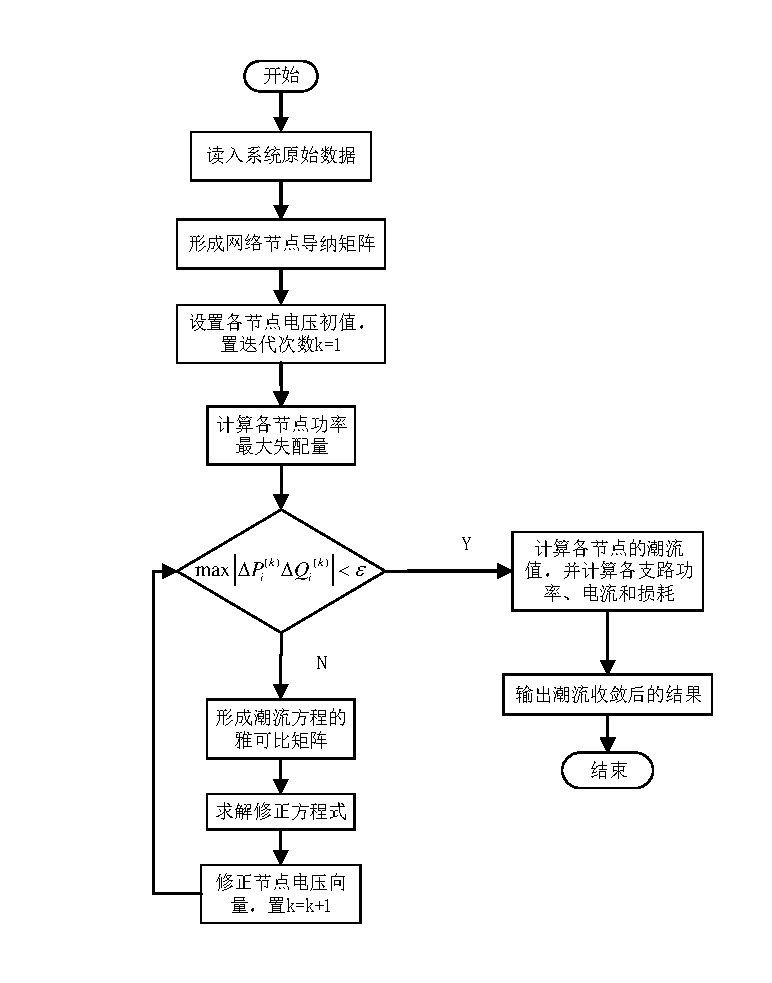
\includegraphics[]{powerFlow.pdf}
  \caption{稳态潮流计算流程图}
  \label{fig:powerFlow}
\end{figure}


在电力系统中,稳定裕度是指系统中各元件的运行状态值与临界状态值的相对距离,表征的是电力系统当前运行状态距离失稳状态的程度。

在电力系统状态脆弱性研究分析中,电力系统的节点电压是研究系统脆弱性的重要指标,电力系统各节点电压的高低实际反映的是电力系统是否正常供电。在电力系统运行过程中,保证
电压的稳定可以有效提高电力系统的运行效率,降低系统出现级联停电的可能性;除此之外,在电力系统状态研究中,负荷节点容量也是一项重要的研究指标,从大规模的停电事故中
可以看出,很多事故原因在于电力系统局部负荷过载,保证电力系统负荷节点的负荷功率在安全容量范围内,可以有效降低因局部负荷过载和级联效应而导致电力系统瘫痪事故发生的
可能性。因此,本文提出电压裕度指标和功率稳定裕度指标作为评估电力系统各元件脆弱性的指标。

在电力系统运行过程中,通过比较节点实际的运行电压和临界电压之间的裕度来评估电网各节点的状态脆弱性。定义“电压裕度”指标如下:
\begin{equation}
\label{equ:chap3:SV}
  S_V=\frac{\left|U_{C}-U_{I}\right|}{\left|\alpha U_{m}\right|}
\end{equation}

式中,$U_C$为电压临界值,$U_I$为当前运行电压值,$\left|\alpha U_{m}\right|$为电压稳定阈值,$\alpha$为电压最大允许的波动率(偏差率)。$U_m$为负荷节点额定电压值。
电压裕度越小,说明系统元件在运行过程中极易达到失稳状态,其脆弱性越强。


在功率稳定裕度指标研究方面,本文的主要专注点在于节点所能承受最大负荷的能力,因此,通过连续潮流(CPF)计算得到各节点的最大负荷功率,并定义“功率稳定裕度”指标如下:
\begin{equation}
\label{equ:chap3:SC}
  S_C=\left|C_M-C_i\right|
  \end{equation}

式中,$C_M$为节点最大负荷功率,$C_i$为节点的额定功率。
功率稳定裕度越小,说明系统元件承受负荷的能力越小,系统越脆弱。

灵敏度的物理意义为:控制量每变动一个单位引起的输出量的变化值。

在电力系统中,灵敏度一般是指以输出或状态向量表征的系统运行状况对控制向量和扰动向量变化的敏感程度。灵敏度分析大部分是建立在潮流方程基础上的,不同学术文献中所用到方法
的不同之处,除了在所提出的评价指标的差别外,还体现在潮流计算中对所用变量的分类和其相互关系的处理上。
基于潮流计算的灵敏度分析的基本方程是节点功率平衡方程,其极坐标形式如下:
\begin{equation}
  \left\{\begin{array}{l}{P_{i}=U_{i} \sum_{j=1}^{n} U_{j}\left(G_{i j} \cos \theta_{i j}+B_{i j} \sin \theta_{i j}\right)} \\ 
{Q_{i}=U_{i} \sum_{j=1}^{n} U_{j}\left(G_{i j} \sin \theta_{i j}-B_{i j} \cos \theta_{i j}\right)}\end{array}\right.  
\end{equation}

在灵敏度分析中,按照各变量的数学作用,可将变量分为如下四类:

$(1)$独立参数向量$\alpha$:包括线路导纳参数$G$,$B$等常量;

$(2)$状态参数向量:$S=\left[U_{l}, \theta_{l}, Q_{g}, \theta_{g}, P_{0}, Q_{0}\right]^{T}$,(潮流计算待求量)包括负荷节点的电压、相位;发电节点的无功功率、相位,
平衡节点的有功功率、无功功率;

$(3)$控制参数向量:$C=\left[P_{l}, Q_{l}, P_{g}, V_{g}, \theta_{0}, U_{0}, B, G \cdots\right]^{T}$(电网模型数据给定(输入)量)包括负荷节点的有功功率和无功功率,
发电节点的有功功率和电压幅值,平衡节点的相角和电压幅值,以及电网支路的导纳和电纳参数等;

$(4)$输出参数向量:$Y=\left[Q_{g}, P_{0}, Q_{0}, P_{L O S S}, Q_{L O S S} \cdots\right]^{T}$,(潮流计算输出量计算结果)包括平衡节点的有功功率和无功功率,以及电网
的有功损耗和无功损耗等。

下标$l$,$g$和$0$表示所对应的量为$PQ$节点,$PV$节点和平衡节点。

在电网指标的研究中,状态参数向量也可以归为输出参数向量中,作为状态脆弱性指标研究的重要参考。

按照以上变量的划分,灵敏度分析的数学方程可以表示为:
\begin{equation}
\left\{\begin{array}{l}{F(S, C, \alpha)=0} \\ {Y=G(S, C, \alpha)}\end{array}\right.
\end{equation}

在上式中,定义$F(S, C, \alpha)=0$为状态方程,包括电力系统中各节点的功率平衡方程,与式3.9等价;定义$Y=G(S, C, \alpha)$为输出方程,包含$PV$节点的无功功率方程、网损方程、
平衡节点方程、支路潮流方程等输出方程。

由于电力系统网络的复杂性,以及潮流状态方程为非线性方程,因而只能用迭代方法求其数值解,所以本文在灵敏度研究分析上,采用简便灵敏度分析方法,简化灵敏度分析过程,忽略潮流方程
变量之间的相互关系,借助牛顿潮流计算方法对其进行迭代求解。在状态方程和输出方程中对控制向量$U$求全微分:
\begin{equation}
  \frac{\partial F}{\partial S} \cdot \frac{d S}{d C}+\frac{\partial F}{\partial C}=0
  \end{equation}
\begin{equation}
  \frac{d Y}{d C}=\frac{\partial G}{\partial S} \cdot \frac{d S}{d C}+\frac{\partial G}{\partial C}
  \end{equation}

从式$3.11$中,可得到状态参数的灵敏度表达式:
\begin{equation}
  \frac{d S}{d C}=-\left(\frac{\partial F}{\partial S}\right)^{-1} \frac{\partial F}{\partial C}
  \end{equation}
  
将式$3.13$代入式$3.12$可得到输出参数的灵敏度表达式:
\begin{equation}
  \frac{d Y}{d C}=-\frac{\partial G}{\partial S}\left(\frac{\partial F}{\partial S}\right)^{-1} \frac{\partial F}{\partial C}+\frac{\partial G}{\partial C}
  \end{equation}

从以上的状态方程和输出方程可以看出,灵敏度指标从不同的变量来考虑可以构造出不同的灵敏度指标。

在电力系统状态指标的研究中,电网损耗指标是电力生产中的重要技术经济指标,它直接反映的是电网整体的能效水平。理论上讲,电网线损率高意味着电力建设落后、网架结构薄弱、
设备老化严重。因此,本文研究负荷节点的功率变化对系统支路功率损耗的影响程度,不仅可以为降低电网损耗率提供参考意见,还能识别出导致电力系统损耗率较高的关键元件。

根据式3.16,对电网损耗灵敏度表达式进行如下定义:
\begin{equation}
  \frac{d P_{LOSS}}{d P_i}=-\frac{\partial G}{\partial S}\left(\frac{\partial F}{\partial S}\right)^{-1} \frac{\partial F}{\partial P_i}+\frac{\partial G}{\partial P_i}
  \end{equation}

式中,$P_{LOSS}$为系统支路损耗,$P_l$为负荷节点功率。

本文就电网有功损耗对灵敏度表达式进行推导,电网有功损耗的表达式:
\begin{equation}
  P_{L O S S}=\sum_{i=1}^{n} \sum_{j=1}^{n} U_{i j}^{2} G_{i j}
  \end{equation}

式中$U_ij$为节点$i$和节点$j$的电压差,$G_ij$为节点$i$和节点$j$电导矩阵。

令$$I_j = \sum_{j=1}^{n} U_{j}\left(G_{i j} \cos \theta_{i j}+B_{i j} \sin \theta_{i j}\right)$$
$$I_i = \sum_{i=1}^{n} U_{i}\left(G_{i j} \cos \theta_{i j}-B_{i j} \sin \theta_{i j}\right)$$

根据式3.11节点功率方程式可得:
\begin{equation}
  \frac{d P_{\text {Loss}}}{d P_{i}}=2 G_{i j} \sum_{i=1}^{n} \sum_{j=1}^{n}\left[\left(\frac{P_{i}}{I_{J}^{2}}-\frac{P_{j}}{I_{I} \cdot I_{J}}\right)\right]
  \end{equation}

从上式可以看出,电网有功损耗对负荷节点的灵敏度不仅和节点注入的有功功率有直接关系,还与电网其他的控制向量参数和状态向量参数有关。所以灵敏度指标是在潮流计算的基础上得出的。

本文所采用的潮流计算方法为牛顿潮流法,这是一种求解非线性代数方程的一种有效且收敛速度快的迭代计算方法。根据节点功率平衡方程式,通过泰勒级数展开保留一阶导数部分,不断进行迭代,
缩小精确解和近似解之间的误差,直到满足精度要求为止。



基于前面的状态脆弱性指标的研究,本节已$IEEE39$电力系统数据集为例,通过连续潮流计算分别计算电力系统节点的最大负荷功率和节点功率变化对电网支路损耗的灵敏度,如图\ref{fig:senseTest}
所示。
\begin{figure}[H] 
  \centering
  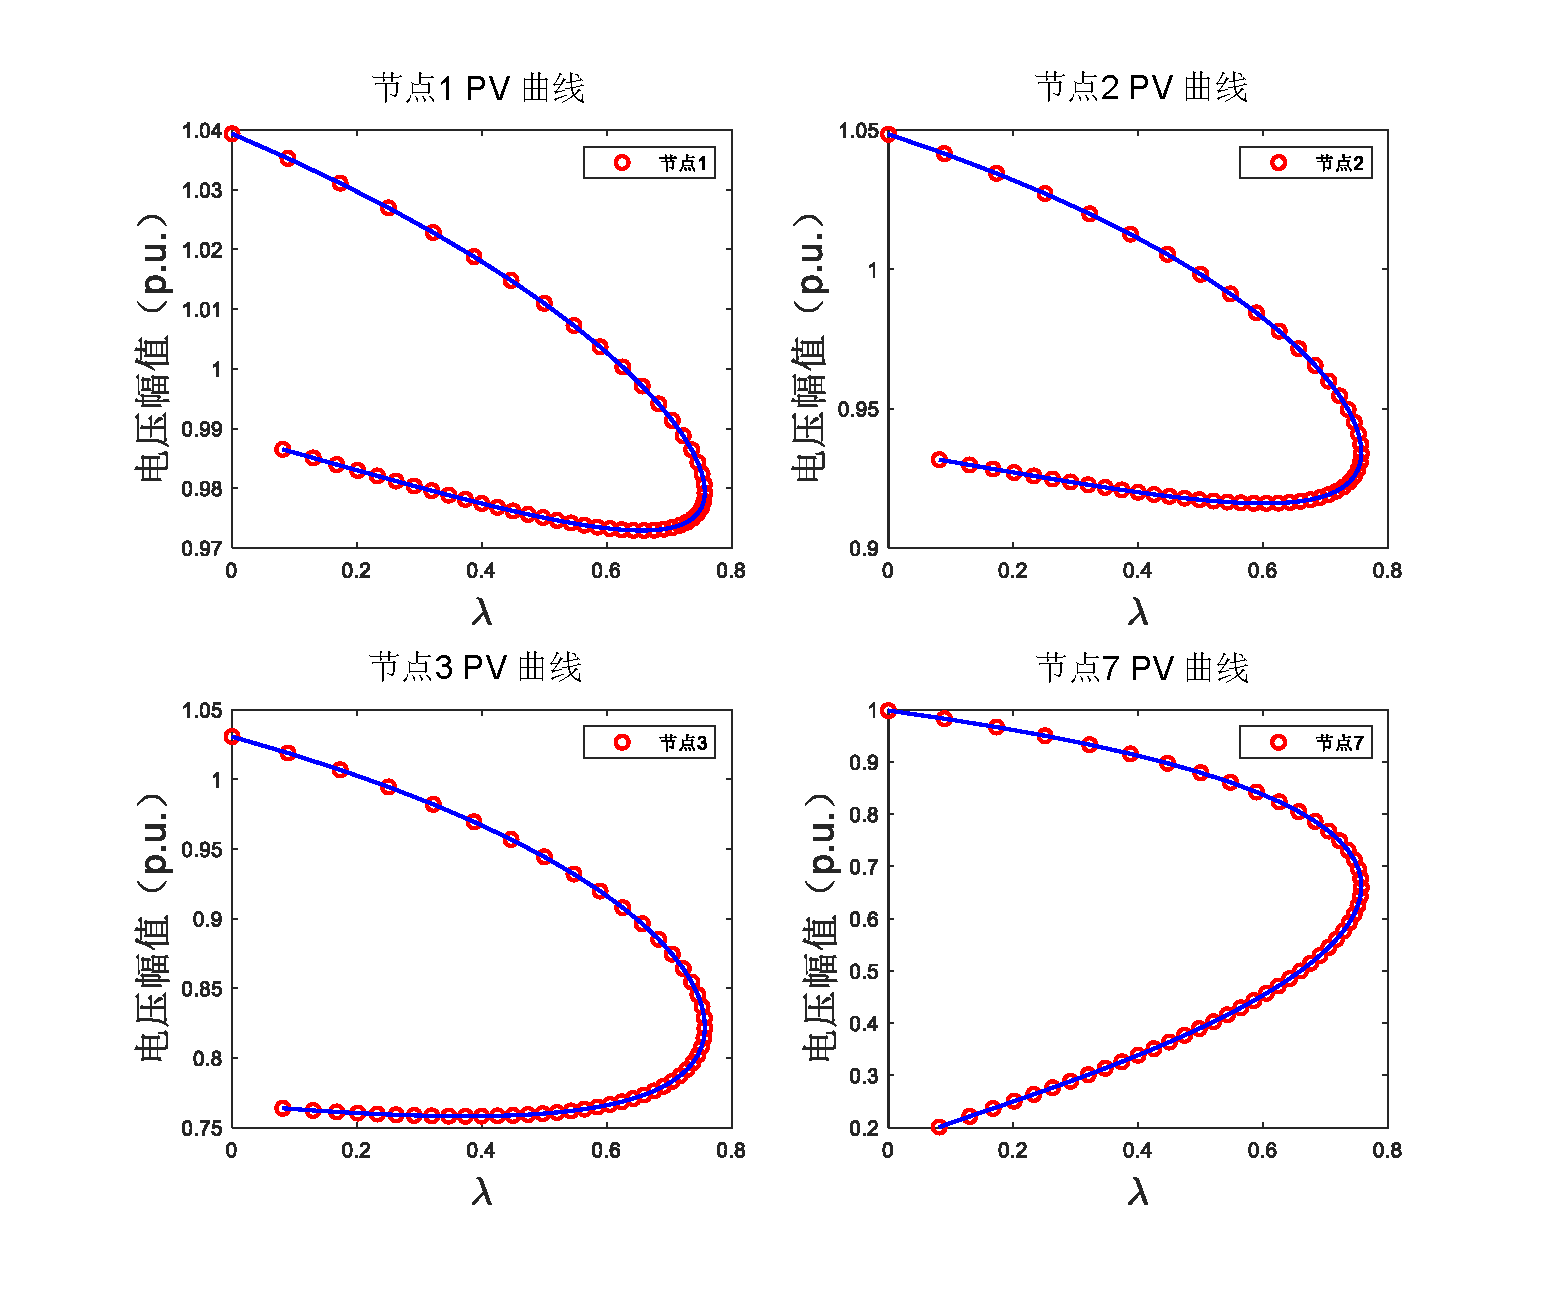
\includegraphics[height=9cm]{PV_curve.pdf}
  \caption{$IEEE39$连续潮流下PV特性曲线}
  \label{fig:PV_curve}
\end{figure}

如图\ref{fig:PV_curve}所示,$\lambda$为负荷增长率,随节点负荷的缓慢增加,不断求解潮流方程,从而描绘出系统的PV曲线。也就是说,鞍岔分节点为电力系统节点电压和功率的临界点。
可以看出,在连续潮流(CPF)计算结果中,系统中不同节点其临界电压和最大节点负荷功率不同,从而在侧面体现出电力系统的异质性。为了方便度量,在负荷增加的方式上采用的是增加负荷增长率的方式,
虽然不同节点的最大负荷增长率相同,但是其最大节点功率负荷不同。具体的临界数据如表\ref{tab:chap3:Critical}所示。
\begin{table}[H]
  \centering
  \caption{节点1、2、3、7临界电压值和最大节点有功功率值}
  \label{tab:chap3:Critical}
  \begin{tabular}{C{4cm}C{2cm}C{2cm}C{2cm}C{2cm}}
  \toprule
  \textbf{节点名} & \textbf{节点1} & \textbf{节点2} & \textbf{节点3} & \textbf{节点7}\\
      \midrule
      节点电压临界值(p.u.)   & 0.979     &0.937       &0.829      &0.660\\
      最大节点有功功率(MW)     & 208.44     &0    &687.68      &499.3\\
  \bottomrule
  \end{tabular}
  \end{table}

在表\ref{tab:chap3:Critical}中,由于节点2为联络节点,注入有功功率和无功功率都给等于零,在电力系统中只是起到连接节点的作用,故在连续潮流(CPF)计算中,将其节点的最大节点负荷设定为零。

\begin{figure}[H] 
  \centering
  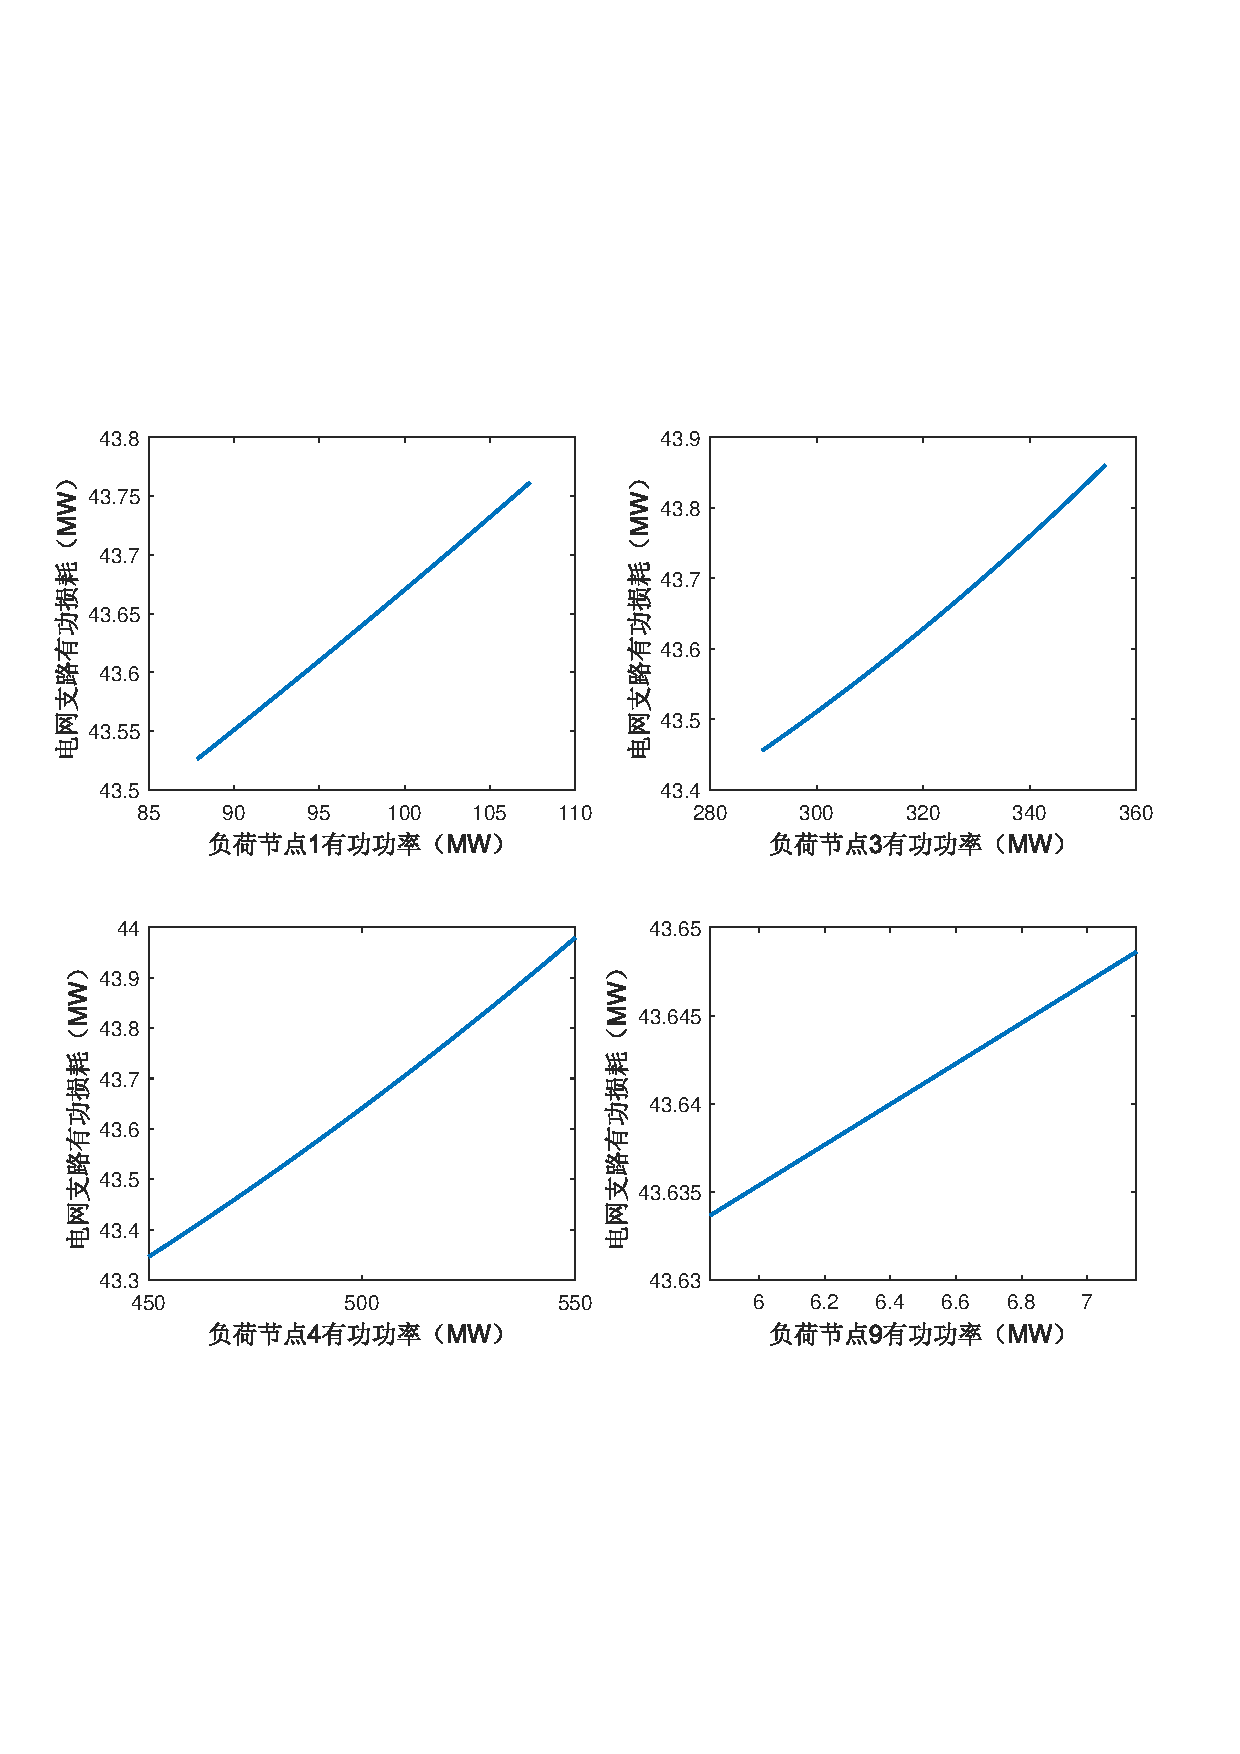
\includegraphics[height=8cm]{senseTest.pdf}
  \caption{$IEEE39$节点1、3、4、9负荷节点灵敏度趋势图}
  \label{fig:senseTest}
\end{figure}

在考虑实际的电网负荷水平的情况下,负荷节点的用电负荷波动不大,故在仿真实验分析时,选取电网负荷节点稳定运行工作点附近的区间进行研究分析,为此,在负荷节点额定功率值的基础上。
取$\pm$10\%的功率区间来进行仿真分析。从图\ref{fig:senseTest}中可以看出,不同节点有功负荷功率的变化对整个系统电网损耗的灵敏度值不同,具体数据如表所示。
\begin{table}[H]
  \centering
  \caption{节点1、3、4、9负荷节点灵敏度值}
  \label{tab:chap3:senseTest}
  \begin{tabular}{C{2cm}C{2cm}C{2cm}C{2cm}C{2cm}}
  \toprule
  \textbf{节点名} & \textbf{节点1} & \textbf{节点3} & \textbf{节点4} & \textbf{节点9}\\
      \midrule
      灵敏度值   & 0.0121     &0.00629       &0.00633     &0.0115 \\
  \bottomrule
  \end{tabular}
  \end{table}

从上表\ref{tab:chap3:senseTest}节点灵敏度数据可以看出,不同节点的灵敏度值差别很大,说明不同负荷节点的在用电负荷变化的情况下,对电网支路的整体损耗不同。根据潮流计算量化结果,
节点1、9、20、23、25、28、29的灵敏度值较大,从网络拓扑位置上看,这些节点大都接近发电节点,从实验结果可以推断出,发电节点向负荷节点的潮流传输线路中,距离发电节点进的负荷节点,在额定
功率平衡点附近的负荷变化对电网支路损耗的影响较大。就灵敏度指标而言,从侧面反映出系统节点的状态脆弱性与系统结构拓扑有一定的联系。




\section{本章小结}
\label{sec:sum3}

本章节通过研究电力系统的稳定性、可靠性和鲁棒性三者之间的区别与联系,得出电力系统的脆弱性本质及脆弱过程,并将给出其数学描述。针对电力系统脆弱性的定义,本文将脆弱性分为结构脆弱性和
状态脆弱性。

在结构脆弱性方面,基于复杂网络理论对电力系统建立了两种模型,一是传统的加权无向图,二是基于$PageRank$算法的无权有向图,分别得到电气度、电气介数和$PR$值脆弱性指标,前两个关注的是支路上
的潮流分布对拓扑的影响,而$PR$值更在意的是有向的链接关系对拓扑的影响。并以 IEEE14 系统为例,使用两种方法建模计算并进行了比较,认为二者分别从不同的角度对拓扑的脆弱性进行了研究,
均具有实际意义。

在状态脆弱性方面,建立了电力系统的负荷模型,选取蒙特卡洛方法作为状态脆弱性的研究方法,基于裕度法和灵敏度法分别定义了电压裕度、功率稳定裕度以及节点负荷灵敏度指标。在此基础上,以$IEEE39$
节点系统为例,就功率稳定裕度和节点负荷灵敏度指标进行仿真分析,为之后的建立电力系统脆弱性量化评估模型奠定了基础。



